\documentclass[fleqn]{article}

\usepackage{graphicx}
\usepackage{xurl}
\usepackage{url}
\usepackage{caption}
\usepackage{fancyhdr}
\usepackage{mathtools}
\usepackage{amsmath}
\usepackage{amssymb}
\usepackage{tikz}
\usepackage{listings}
\usepackage{xcolor}
\usepackage{float}

\definecolor{codegreen}{rgb}{0,0.6,0}
\definecolor{codegray}{rgb}{0.5,0.5,0.5}
\definecolor{codepurple}{rgb}{0.58,0,0.82}
\definecolor{backcolour}{rgb}{0.95,0.95,0.92}

\lstdefinestyle{mystyle}{
	backgroundcolor=\color{backcolour},   
	commentstyle=\color{codegreen},
	keywordstyle=\color{magenta},
	numberstyle=\tiny\color{codegray},
	stringstyle=\color{codepurple},
	basicstyle=\ttfamily\footnotesize,
	breakatwhitespace=false,         
	breaklines=true,                 
	captionpos=b,                    
	keepspaces=true,                 
	numbers=left,                    
	numbersep=5pt,                  
	showspaces=false,                
	showstringspaces=false,
	showtabs=false,                  
	tabsize=2
}

\lstset{style=mystyle}

\usepackage{xepersian}

\settextfont[BoldFont={XB Zar bold.ttf}]{XB Zar.ttf}
\setlength\parindent{0pt}

\title{

\includegraphics[width=0.4\textwidth]{sharif.png}\\
\normalsize{دانشکده مهندسی کامپیوتر}\\
\vspace{1cm}
	
\huge{آزمایشگاه طراحی سیستم‌های دیجیتال}
\\
\Large{گزارش آزمایش دوم}
\\
}

\author{
\\
دکتر سیاوش بیات سرمدی
\\
\\
پارسا محمدیان --- 98102284
}

\date{\today}

\begin{document}

\clearpage\maketitle
\thispagestyle{empty}

\newpage

\pagestyle{fancy}
\lhead{آزمایشگاه طراحی سیستم‌های دیجیتال}

\rhead{پارسا محمدیان}


\tableofcontents

\setcounter{page}{1}

\newpage

\section{مقدمه}

\subsection*{عنوان گزارش}
طراحي مدارهاي تركيبي با استفاده از امكانات شماتيك.
\subsection*{موضوع}
استفاده از نرم‌افزارهای طراحی به کمک کامپیوتر \footnote{\lr{CAD}} و امکانات 
شماتیک آن‌ها برای طراحی و پیاده‌سازی مدار ترکیبی.
\subsection*{شرح ابزارها و برنامه‌های مورد استفاده}
در این آزمایش از نرم‌افزار \lr{ISE Desgin Suite} که محصول شرکت \lr{Xilinx} است 
استفاده کرده‌ام.

\section{چارچوب نظری و شرح آزمایش}
در این آزمایش مداری برای کنترل ورود و خروج به اتاق طراحی کردیم. برای این 
کار از دو شمارنده استفاده کردیم. یکی برای نگه داشتن تعداد افراد حاضر در 
اتاق و دیگری برای نگه داشتن زمان باز ماندن در ورودی. به دلیل کوچک بودن 
مدار، این ماژول‌ها در خود ماژول اصلی آمده‌اند. تمامی کدها در ماژول اصلی 
\lr{Main.v} وجود دارند.

\section{گزارش متنی}
\begin{latin}
\begin{lstlisting}[basicstyle=\tiny]
Release 14.7 - xst P.20131013 (nt64)
Copyright (c) 1995-2013 Xilinx, Inc.  All rights reserved.
--> Parameter TMPDIR set to xst/projnav.tmp


Total REAL time to Xst completion: 0.00 secs
Total CPU time to Xst completion: 0.15 secs

--> Parameter xsthdpdir set to xst


Total REAL time to Xst completion: 0.00 secs
Total CPU time to Xst completion: 0.15 secs

--> Reading design: Main.prj

TABLE OF CONTENTS
1) Synthesis Options Summary
2) HDL Compilation
3) Design Hierarchy Analysis
4) HDL Analysis
5) HDL Synthesis
5.1) HDL Synthesis Report
6) Advanced HDL Synthesis
6.1) Advanced HDL Synthesis Report
7) Low Level Synthesis
8) Partition Report
9) Final Report
9.1) Device utilization summary
9.2) Partition Resource Summary
9.3) TIMING REPORT


=========================================================================
*                      Synthesis Options Summary                        *
=========================================================================
---- Source Parameters
Input File Name                    : "Main.prj"
Input Format                       : mixed
Ignore Synthesis Constraint File   : NO

---- Target Parameters
Output File Name                   : "Main"
Output Format                      : NGC
Target Device                      : xc3sd3400a-4-fg676

---- Source Options
Top Module Name                    : Main
Automatic FSM Extraction           : YES
FSM Encoding Algorithm             : Auto
Safe Implementation                : No
FSM Style                          : LUT
RAM Extraction                     : Yes
RAM Style                          : Auto
ROM Extraction                     : Yes
Mux Style                          : Auto
Decoder Extraction                 : YES
Priority Encoder Extraction        : Yes
Shift Register Extraction          : YES
Logical Shifter Extraction         : YES
XOR Collapsing                     : YES
ROM Style                          : Auto
Mux Extraction                     : Yes
Resource Sharing                   : YES
Asynchronous To Synchronous        : NO
Use DSP Block                      : Auto
Automatic Register Balancing       : No

---- Target Options
Add IO Buffers                     : YES
Global Maximum Fanout              : 500
Add Generic Clock Buffer(BUFG)     : 24
Register Duplication               : YES
Slice Packing                      : YES
Optimize Instantiated Primitives   : NO
Use Clock Enable                   : Yes
Use Synchronous Set                : Yes
Use Synchronous Reset              : Yes
Pack IO Registers into IOBs        : Auto
Equivalent register Removal        : YES

---- General Options
Optimization Goal                  : Speed
Optimization Effort                : 1
Keep Hierarchy                     : No
Netlist Hierarchy                  : As_Optimized
RTL Output                         : Yes
Global Optimization                : AllClockNets
Read Cores                         : YES
Write Timing Constraints           : NO
Cross Clock Analysis               : NO
Hierarchy Separator                : /
Bus Delimiter                      : <>
Case Specifier                     : Maintain
Slice Utilization Ratio            : 100
BRAM Utilization Ratio             : 100
DSP48 Utilization Ratio            : 100
Verilog 2001                       : YES
Auto BRAM Packing                  : NO
Slice Utilization Ratio Delta      : 5

=========================================================================


=========================================================================
*                          HDL Compilation                              *
=========================================================================
Compiling verilog file "Main.v" in library work
Module <Main> compiled
No errors in compilation
Analysis of file <"Main.prj"> succeeded.


=========================================================================
*                     Design Hierarchy Analysis                         *
=========================================================================
Analyzing hierarchy for module <Main> in library <work>.


=========================================================================
*                            HDL Analysis                               *
=========================================================================
Analyzing top module <Main>.
Module <Main> is correct for synthesis.


=========================================================================
*                           HDL Synthesis                               *
=========================================================================

Performing bidirectional port resolution...

Synthesizing Unit <Main>.
Related source file is "Main.v".
Found 1-bit register for signal <close>.
Found 1-bit register for signal <in>.
Found 1-bit register for signal <open>.
Found 1-bit register for signal <out>.
Found 1-bit register for signal <keepOpen>.
Found 4-bit up counter for signal <members>.
Found 4-bit addsub for signal <members$mux0000>.
Found 4-bit comparator less for signal <old_keepOpen_2$cmp_lt0000> created at 
line 36.
Found 4-bit comparator greatequal for signal <open$cmp_ge0000> created at line 
36.
Found 2-bit up counter for signal <waitOpen>.
Summary:
inferred   2 Counter(s).
inferred   5 D-type flip-flop(s).
inferred   1 Adder/Subtractor(s).
inferred   2 Comparator(s).
Unit <Main> synthesized.

INFO:Xst:1767 - HDL ADVISOR - Resource sharing has identified that some 
arithmetic operations in this design can share the same physical resources for 
reduced device utilization. For improved clock frequency you may try to disable 
resource sharing.

=========================================================================
HDL Synthesis Report

Macro Statistics
# Adders/Subtractors                                   : 1
4-bit addsub                                          : 1
# Counters                                             : 2
2-bit up counter                                      : 1
4-bit up counter                                      : 1
# Registers                                            : 5
1-bit register                                        : 5
# Comparators                                          : 2
4-bit comparator greatequal                           : 1
4-bit comparator less                                 : 1

=========================================================================

=========================================================================
*                       Advanced HDL Synthesis                          *
=========================================================================


=========================================================================
Advanced HDL Synthesis Report

Macro Statistics
# Adders/Subtractors                                   : 1
4-bit addsub                                          : 1
# Counters                                             : 2
2-bit up counter                                      : 1
4-bit up counter                                      : 1
# Registers                                            : 5
Flip-Flops                                            : 5
# Comparators                                          : 2
4-bit comparator greatequal                           : 1
4-bit comparator less                                 : 1

=========================================================================

=========================================================================
*                         Low Level Synthesis                           *
=========================================================================

Optimizing unit <Main> ...

Mapping all equations...
Building and optimizing final netlist ...
Found area constraint ratio of 100 (+ 5) on block Main, actual ratio is 0.

Final Macro Processing ...

=========================================================================
Final Register Report

Macro Statistics
# Registers                                            : 11
Flip-Flops                                            : 11

=========================================================================

=========================================================================
*                           Partition Report                            *
=========================================================================

Partition Implementation Status
-------------------------------

No Partitions were found in this design.

-------------------------------

=========================================================================
*                            Final Report                               *
=========================================================================
Final Results
RTL Top Level Output File Name     : Main.ngr
Top Level Output File Name         : Main
Output Format                      : NGC
Optimization Goal                  : Speed
Keep Hierarchy                     : No

Design Statistics
# IOs                              : 7

Cell Usage :
# BELS                             : 21
#      INV                         : 2
#      LUT2                        : 3
#      LUT2_D                      : 1
#      LUT2_L                      : 1
#      LUT3                        : 1
#      LUT4                        : 9
#      LUT4_L                      : 1
#      MUXF5                       : 2
#      VCC                         : 1
# FlipFlops/Latches                : 11
#      FDE                         : 4
#      FDR                         : 4
#      FDRE                        : 3
# Clock Buffers                    : 1
#      BUFGP                       : 1
# IO Buffers                       : 6
#      IBUF                        : 2
#      OBUF                        : 4
=========================================================================

Device utilization summary:
---------------------------

Selected Device : 3sd3400afg676-4 

Number of Slices:                       12  out of  23872     0%  
Number of Slice Flip Flops:             11  out of  47744     0%  
Number of 4 input LUTs:                 18  out of  47744     0%  
Number of IOs:                           7
Number of bonded IOBs:                   7  out of    469     1%  
Number of GCLKs:                         1  out of     24     4%  

---------------------------
Partition Resource Summary:
---------------------------

No Partitions were found in this design.

---------------------------


=========================================================================
TIMING REPORT

NOTE: THESE TIMING NUMBERS ARE ONLY A SYNTHESIS ESTIMATE.
FOR ACCURATE TIMING INFORMATION PLEASE REFER TO THE TRACE REPORT
GENERATED AFTER PLACE-and-ROUTE.

Clock Information:
------------------
-----------------------------------+------------------------+-------+
Clock Signal                       | Clock buffer(FF name)  | Load  |
-----------------------------------+------------------------+-------+
clk                                | BUFGP                  | 11    |
-----------------------------------+------------------------+-------+

Asynchronous Control Signals Information:
----------------------------------------
No asynchronous control signals found in this design

Timing Summary:
---------------
Speed Grade: -4

Minimum period: 4.179ns (Maximum Frequency: 239.292MHz)
Minimum input arrival time before clock: 4.168ns
Maximum output required time after clock: 5.531ns
Maximum combinational path delay: No path found

Timing Detail:
--------------
All values displayed in nanoseconds (ns)

=========================================================================
Timing constraint: Default period analysis for Clock 'clk'
Clock period: 4.179ns (frequency: 239.292MHz)
Total number of paths / destination ports: 82 / 21
-------------------------------------------------------------------------
Delay:               4.179ns (Levels of Logic = 2)
Source:            members_2 (FF)
Destination:       out (FF)
Source Clock:      clk rising
Destination Clock: clk rising

Data Path: members_2 to out
Gate     Net
Cell:in->out      fanout   Delay   Delay  Logical Name (Net Name)
----------------------------------------  ------------
FDE:C->Q              8   0.591   0.900  members_2 (members_2)
LUT2_D:I0->LO         1   0.648   0.103  Mcount_members111 (N15)
LUT4:I3->O            1   0.648   0.420  out_or000011 (out_or0000)
FDR:R                     0.869          out
----------------------------------------
Total                      4.179ns (2.756ns logic, 1.423ns route)
(65.9% logic, 34.1% route)

=========================================================================
Timing constraint: Default OFFSET IN BEFORE for Clock 'clk'
Total number of paths / destination ports: 22 / 12
-------------------------------------------------------------------------
Offset:              4.168ns (Levels of Logic = 3)
Source:            ent (PAD)
Destination:       members_0 (FF)
Destination Clock: clk rising

Data Path: ent to members_0
Gate     Net
Cell:in->out      fanout   Delay   Delay  Logical Name (Net Name)
----------------------------------------  ------------
IBUF:I->O             3   0.849   0.674  ent_IBUF (ent_IBUF)
LUT4:I0->O            2   0.648   0.450  open_not00011 (open_not0001)
LUT4:I3->O            4   0.648   0.587  members_not00011 (members_not0001)
FDE:CE                    0.312          members_0
----------------------------------------
Total                      4.168ns (2.457ns logic, 1.711ns route)
(58.9% logic, 41.1% route)

=========================================================================
Timing constraint: Default OFFSET OUT AFTER for Clock 'clk'
Total number of paths / destination ports: 4 / 4
-------------------------------------------------------------------------
Offset:              5.531ns (Levels of Logic = 1)
Source:            in (FF)
Destination:       in (PAD)
Source Clock:      clk rising

Data Path: in to in
Gate     Net
Cell:in->out      fanout   Delay   Delay  Logical Name (Net Name)
----------------------------------------  ------------
FDR:C->Q              1   0.591   0.420  in (in_OBUF)
OBUF:I->O                 4.520          in_OBUF (in)
----------------------------------------
Total                      5.531ns (5.111ns logic, 0.420ns route)
(92.4% logic, 7.6% route)

=========================================================================


Total REAL time to Xst completion: 4.00 secs
Total CPU time to Xst completion: 4.45 secs

--> 

Total memory usage is 4514000 kilobytes

Number of errors   :    0 (   0 filtered)
Number of warnings :    0 (   0 filtered)
Number of infos    :    1 (   0 filtered)
\end{lstlisting}
\end{latin}

\section{فرکانس کاری مدار}
همانطور که در خط 323 گزارش متنی مشخص است، \lr{Delay} مدار 4/179 نانو ثانیه 
است. 
$$
f = \frac{1}{4.179ns \times 10^{-9}} \approxeq 0.239 \times 10^9 Hz 
= 239 MHz
$$
پس فرکانس کاری 191 مگاهرتز است. 

\section{تست مدار}
تستی برای بررسی صحت عملکرد مدار در فایل 
\lr{MainTest.v}
نوشته شده است که اتاق را پر میکند و همچین حالت‌های لبه‌ای (خروجی در صورت خالی 
بودن اتاق و ورود در صورت پر بودن اتاق) را هم چک می‌کند.

\section{شماتیک}
\begin{figure}[H]
	\centering
	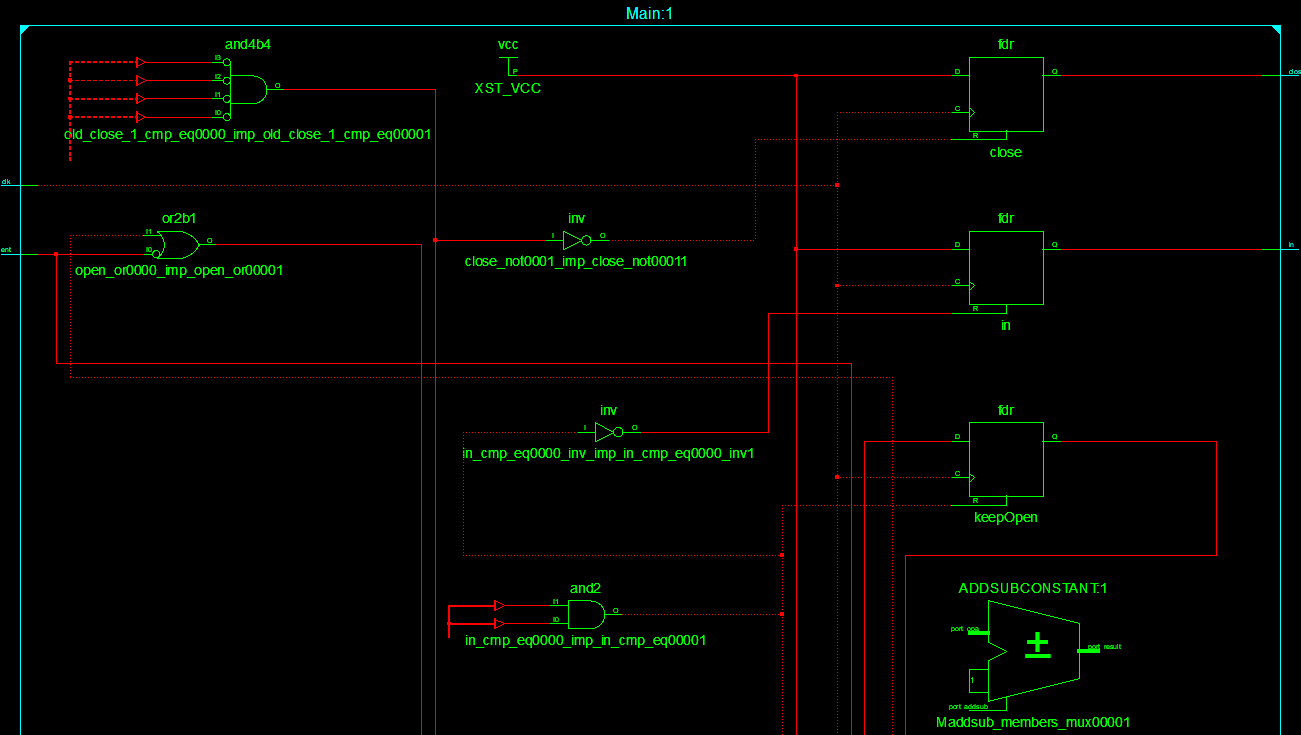
\includegraphics[width=.5\paperwidth]{./Schematic/1.png}
\end{figure}
\begin{figure}[H]
	\centering
	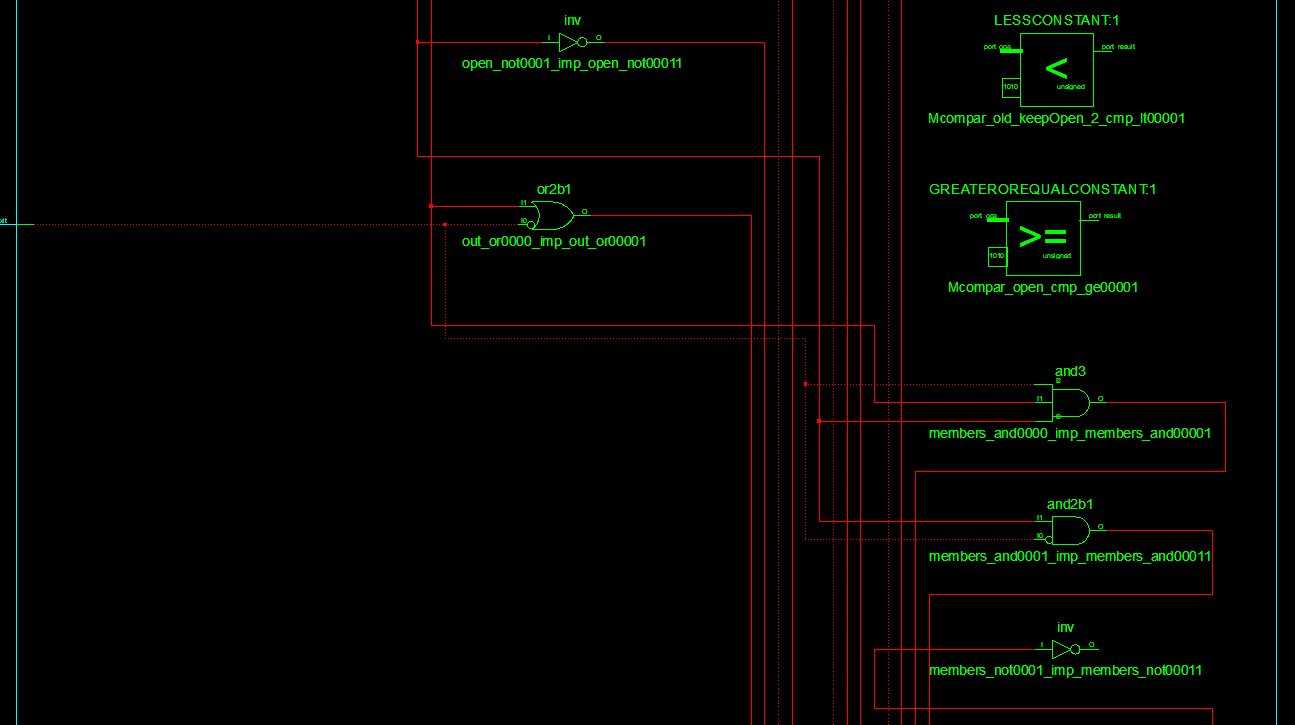
\includegraphics[width=.5\paperwidth]{./Schematic/2.png}
\end{figure}
\begin{figure}[H]
	\centering
	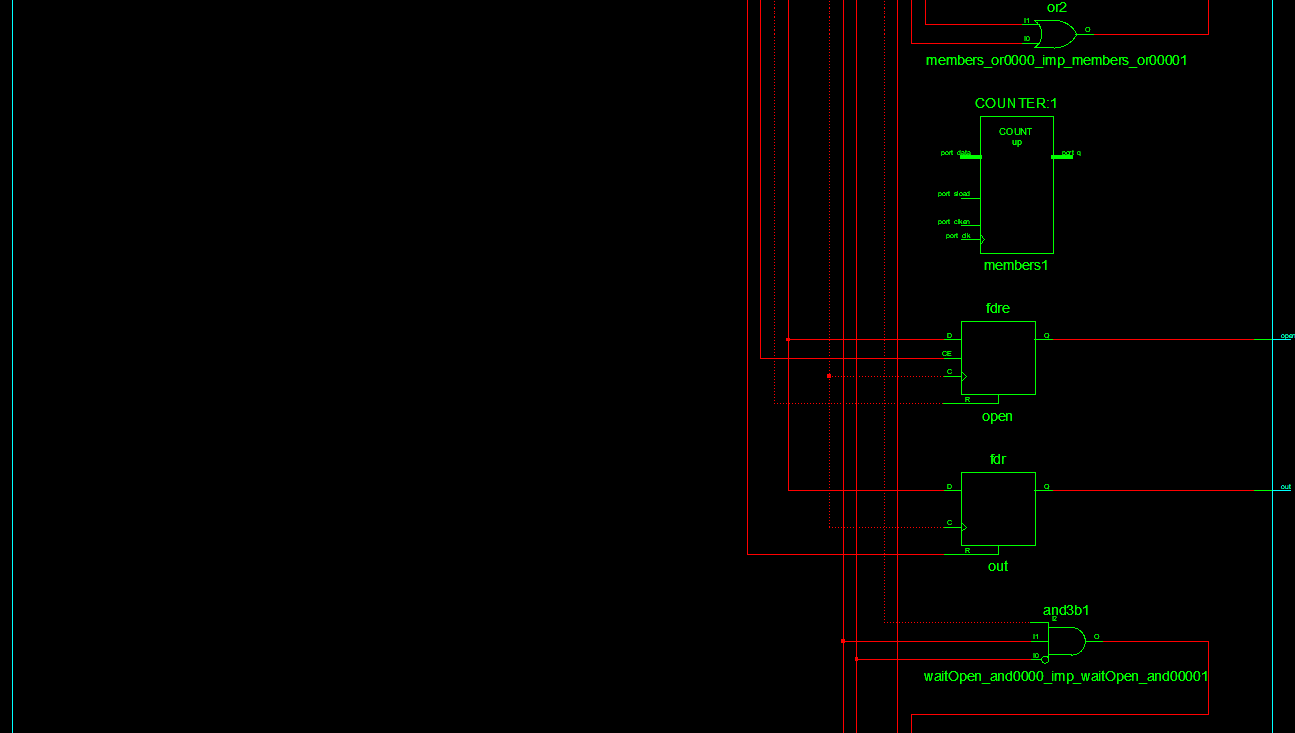
\includegraphics[width=.5\paperwidth]{./Schematic/3.png}
\end{figure}
\begin{figure}[H]
	\centering
	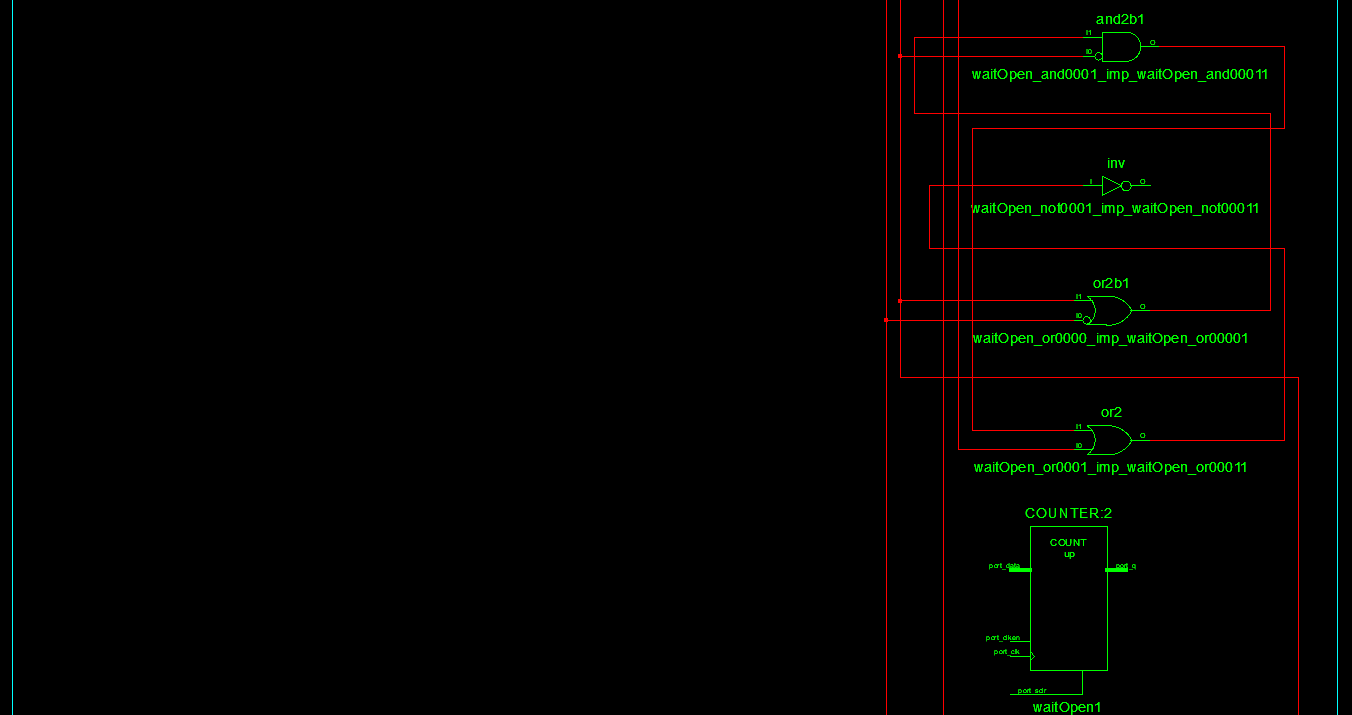
\includegraphics[width=.5\paperwidth]{./Schematic/4.png}
\end{figure}
\begin{figure}[H]
	\centering
	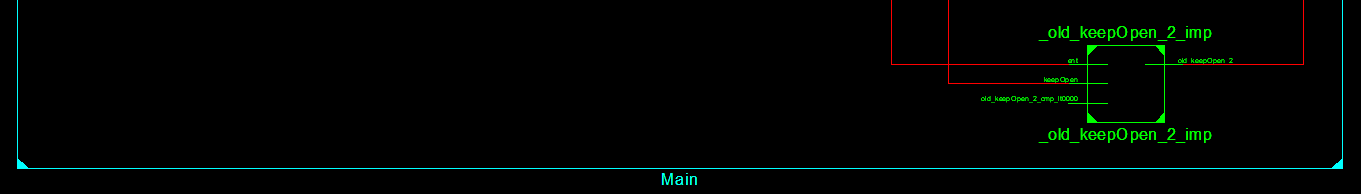
\includegraphics[width=.5\paperwidth]{./Schematic/5.png}
\end{figure}

\end{document}
